\documentclass[10pt,a4paper]{article}
\usepackage[utf8]{inputenc}
\usepackage[T1]{fontenc}
\usepackage{amsmath}
\usepackage{amssymb}
\usepackage{graphicx}
\usepackage{nicematrix}
\usepackage[left=2.00cm, right=2.00cm, top=2.00cm, bottom=2.00cm]{geometry}
\usepackage{float}
\usepackage{caption}
\usepackage{subcaption}
\usepackage{color}
\usepackage[
	colorlinks=true,
	linkcolor=blue,
	filecolor=blue,      
	urlcolor=cyan,
	citecolor=cyan,    
]{hyperref}

\title{\textbf{CIE6107 - Robotics and Intelligent Systems \\Assignment 1}}
\author{Zixing JIANG}
\begin{document}
	
\begin{flushleft}
	CSC3180: Fundamentals of Artificial Intelligence, Spring 2023\\
	Project Proposal, Group 10\\
	\today
\end{flushleft}
	
\begin{flushright}\vspace{-18mm}
	
\includegraphics[height=1.7cm]{figure/logo.png}
\end{flushright}
	
\begin{center}\vspace{0.5cm}
	\textbf{\Large Adaptive Dynamic Stabilization of a Self-Balancing Scooter}\\~\\
	\large Hongyi Yang, Muhan Lin, Xuanyang Xu, Zixing Jiang
\end{center}
{\noindent}\rule{\linewidth}{0.1mm}

\section{Introduction}
The self-balancing scooter (Figure \ref{fig:scooter}) is a common urban commuter tool. One of the most critical features in self-balancing scooter is dynamic stabilization,  which allows the scooter to maintain its balance while in motion. Without this feature, it would be very difficult for riders to stay upright and control the scooter, and even cause safety accidents in severe cases. In order to achieve dynamic stabilization, the traditional automatic control methods, including Proportional-Integral-Derivative (PID) control and Model Predictive Control (MPC), model the self-balancing scooter as a cart-pole system (Figure \ref{fig:cart-pole}) and designs the controller by deriving its system dynamics. However, the dynamics-based control is sensitive to the rider's weight and center of mass (CoM). For riders of different weights and CoMs, the performance of stabilization varies. In this project, we aim to utilize the learning ability of artificial intelligence to design a dynamic stabilizer that adapts to different rider weights and CoMs.

\begin{figure}[H]
	\centering
	\begin{subfigure}[b]{0.3\textwidth}
		\centering
		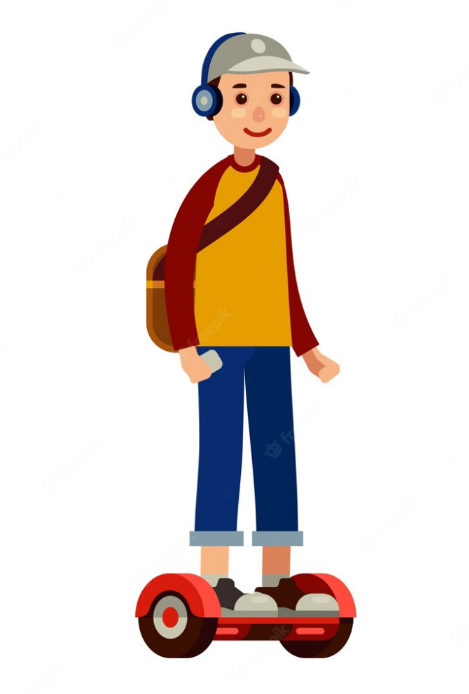
\includegraphics[width=0.5\textwidth]{figure/scooter}
		\caption{Man on a self-balancing scooter}
		\label{fig:scooter}
	\end{subfigure}
	\hfill
	\begin{subfigure}[b]{0.3\textwidth}
		\centering
		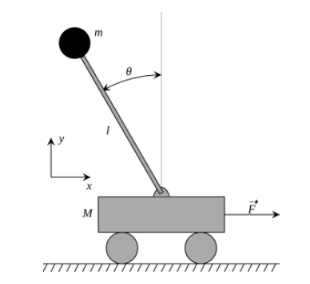
\includegraphics[width=0.85\textwidth]{figure/cart-pole}
		\caption{Cart-pole system dynamics}
		\label{fig:cart-pole}
	\end{subfigure}
	\hfill
	\begin{subfigure}[b]{0.3\textwidth}
		\centering
		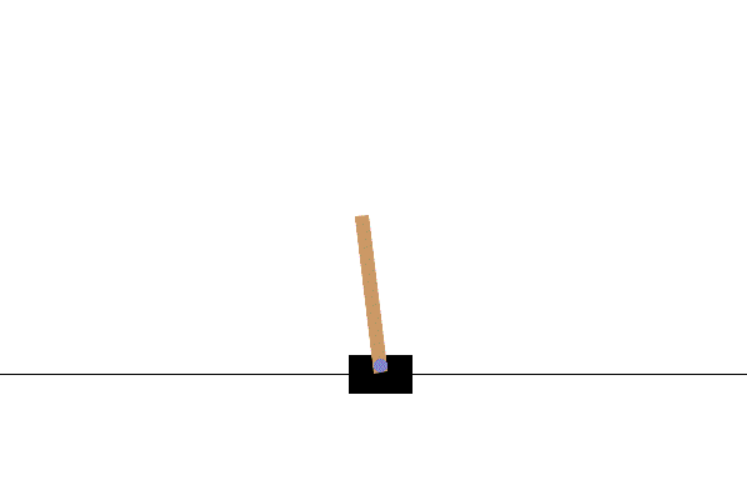
\includegraphics[width=\textwidth]{figure/open-ai}
		\caption{OpenAI Cart Pole Environment}
		\label{fig:openai}
	\end{subfigure}
	\caption{Illustrations of (a) the self-balancing scooter, (b) the cart-pole system dynamics, and (c) the OpenAI Cart Pole environment.}
	\label{fig:three graphs}
\end{figure}

\section{Problem Statement}
In this project, we model the scooter as the cart-pole system (Figure \ref{fig:cart-pole}). The wheel of scooter is the cart the rider-scooter mass is the pole. Then the adaptive stabilization problem can be formulated as follows: control the inclination ($\theta$) of a pole with \textcolor{red}{varying mass and CoM} within a certain range by controlling the movement ($x$) of the cart (leftward or rightward).  We intend to apply reinforcement learning (RL) to solve this problem. Namely, given the observation of the environment ($\theta, \dot{\theta}, x, \dot{x}$), we want our agent (cart) to learn a policy (move leftward or move rightward) to stable the varying pole through trail and reward. We plan to implement our RL algorithm based on the \href{https://gymnasium.farama.org/environments/classic_control/cart_pole/}{OpenAI Gym environment for cart-pole} (Figure \ref{fig:openai}). 

\section{Work Distribution}
\begin{itemize}
	\item Zixing Jiang: RL algorithm design and implementation
	\item Xuanyang Xu: RL algorithm design and implementation
	\item Muhan Lin: OpenAI Gym environment modification, Algorithm implementation
	\item Hongyi Yang: OpenAI Gym environment modification, Algorithm implementation
\end{itemize}
Report and presentation will be done jointly by all members.
\section{Project Schedule}
\begin{itemize}
	\item Week 9: modify the OpenAI Gym environment according to our needs
	\item Week 10: design and implementation RL algorithms for the adaptive stabilization task
	\item Week 11: design and implementation RL algorithms for the adaptive stabilization task
	\item Week 12: validate and optimize (if possible) our algorithm  
	\item Week 13: record video demo and draft report
	\item Week 14: group presentation
\end{itemize}
\end{document}